%   % !TEX root = ../../VIII,3_Rahmen-TeX_9-0.tex
%  
%   Signatur/Tex-Datei:	LH_37_05_144r-145v
%   RK-Nr. 	57268
%   Überschrift: 	Specimina artis condendi theoremata
%   Titel: 			Specimina artis condendi theoremata
%   Datierung:		(Ende?) Mai 1677 (a. St.?), eigh.
%   WZ: 	im Falz, Nr. 803005 		
%   edlabels:			12		
%   Diagramme: 		3
%
%   NB: 		Auf einem Träger mit 57267_1 und _2 und _3
%
%
%
%
\selectlanguage{ngerman}
\frenchspacing
%
\begin{ledgroupsized}[r]{120mm}
\footnotesize
\pstart
\noindent\textbf{Überlieferung:}
\pend
\end{ledgroupsized}
\begin{ledgroupsized}[r]{114mm}
\footnotesize
\pstart \parindent -6mm 
\makebox[6mm][l]{\textit{L}}% 
%
%
Konzept: LH~XXXVII~5 Bl.~144\textendash145.
Ein Bogen~2\textsuperscript{o};
Wasserzeichen in der Mitte von Bl.~145;
Papiererhaltungsmaßnahmen;
Papierbruch an den Blatträndern mit Textverlust.
%
Eine Seite auf Bl.~145~v\textsuperscript{o} und die Hälfte einer Spalte auf Bl.~144~r\textsuperscript{o}.
Bl.~144~r\textsuperscript{o} überliefert auch N.~\ref{57267_1}.	
Auf Bl.~144~v\textsuperscript{o} und 145~r\textsuperscript{o} sowie im Randbereich von Bl.~144~r\textsuperscript{o} wird zudem N.~\ref{57267_2} überliefert;
die unteren zwei Drittel von Bl.~145~r\textsuperscript{o} und der obere Rand von Bl.~145~v\textsuperscript{o} überliefern N.~\ref{57267_3}.
\pend
\end{ledgroupsized}
%
\begin{ledgroupsized}[r]{114mm}
\footnotesize
\pstart
\parindent -6mm 
\makebox[6mm][l]{\textit{E}}% %%
(tlw.) \textsc{Fichant} 1994, S.~365\textendash367\cite{01056}.
\pend%
\end{ledgroupsized}
%
%
\selectlanguage{latin}
\frenchspacing
%
% \newpage%
\vspace{8mm}
\pstart%
\normalsize%
\noindent%
%
\edlabel{37_05_144r-145v_8a}% zwecks Referenzierung der Randanmerkung
\edtext{\lbrack145~v\textsuperscript{o}\rbrack}{%
\lemma{}%
\Afootnote{%
\textit{Am Rand, über \lbrack\textit{Fig.~1}\rbrack:} %
\textlangle Pri\textrangle oribus paginis\textsuperscript{\lbrack a\rbrack} non per omnia \textlangle h\textrangle aec calculavi, sed haec ultimo demum. Maij 1677.%
\newline\newline%Marginalienapparat:
{\footnotesize \textsuperscript{\lbrack a\rbrack} \textlangle Pri\textrangle oribus paginis: Die ersten drei Seiten des Bogens überliefern N.~\ref{57267_1}, N.~\ref{57267_2} und N.~\ref{57267_3}.}%
}}%
\edlabel{37_05_144r-145v_8b}
\pend%
% Überschrift
\pstart%
\centering%
Specimina artis condendi theoremata
\pend%
\vspace{\baselineskip}
%
\vspace{1.0em}%
%
  \centerline{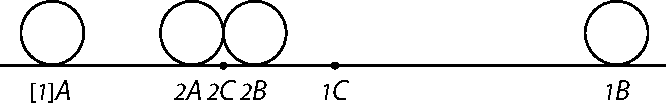
\includegraphics[width=0.65\textwidth]{gesamttex/edit_VIII,3/images/LH_37_05_144r-145v_d1_145v.pdf}} 
    \vspace{0.5em}
\centerline{\lbrack\textit{Fig.~1}\rbrack}
% \newpage%
  \vspace{1.5em}
%
  \vspace{1.0em}
  \centerline{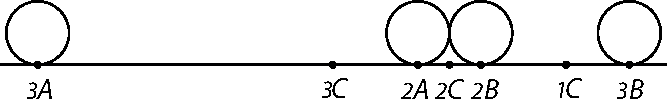
\includegraphics[width=0.65\textwidth]{gesamttex/edit_VIII,3/images/LH_37_05_144r-145v_d2_145v.pdf}} 
    \vspace{0.5em}
\centerline{\lbrack\textit{Fig.~2}\rbrack}
% \newpage%
 % \vspace{2.5em}
\newpage
\pstart\noindent
\hspace{1mm}\hspace{-1mm}% Trick, weil \edlabel nicht zu \par-Beginn sein darf
%
\edlabel{37_05_144r-145v_12a}%
\edtext{}{% zweitelige A-Footnote zu Regula (1) und (2)
{\xxref%
{37_05_144r-145v_12a}{37_05_144r-145v_12b}}%
\lemma{}\Afootnote{%
\textit{Nachträglich zwischen \lbrack Fig.~1\rbrack\ und der ersten Textzeile eingefügt, bezogen auf Regel} (1):\enskip %
(Quod\phantom)\hspace*{-1.2mm} centrum gravitatis\protect\index{Sachverzeichnis}{centrum gravitatis} semper in eadem recta procedit ac demonstrabitur ope concursus gravium et levium in 
aqua,\textsuperscript{\lbrack a\rbrack}\protect\index{Sachverzeichnis}{concursus gravium et levium in aqua} nonnihil
obliqui.\textsuperscript{\lbrack b\rbrack}
Ostenditur enim posito quod centrum gravitatis\protect\index{Sachverzeichnis}{centrum gravitatis} non ita procedat, dari motum
perpetuum\protect\index{Sachverzeichnis}{motus perpetuus}, fingendo gravia et levia prius non connexa mox connecti in libram\protect\index{Sachverzeichnis}{libra}. Idem fiet et sine
liquore, si unum descendat gravitate\protect\index{Sachverzeichnis}{gravitas}, alterum ascendat impulsu, oblique. Demonstrationes tales ex semiphysicis\protect\index{Sachverzeichnis}{demonstratio ex semiphysicis}
quatenus gravitate\protect\index{Sachverzeichnis}{gravitas} utuntur, possunt reddi abstractae, si pro gravitate adhibeat ejus causam\protect\index{Sachverzeichnis}{causa gravitatis}, fingendo motum universalem depellentem\protect\index{Sachverzeichnis}{motus universalis depellens}.\lbrack\phantom(\hspace*{-1.2mm})\rbrack
%
\newline\vspace{-0.5em}\newline%Marginalienapparat:
{\footnotesize 
\textsuperscript{\lbrack a\rbrack} aqua, \textit{(1)}~ob \textit{(2)}~nihi \textit{(3)}~nonnihil~\textit{L}
\textsuperscript{\lbrack b\rbrack} (Quod\phantom)\hspace*{-1.2mm} \lbrack...\rbrack\ obliqui: Ein entsprechender Beweis wird in \textit{De corporum concursu}, \textit{Scheda nona} von Januar 1678 (N.~\ref{dcc_09}) erbracht.}%
\newline\newline % 2. Teil der A-Fn.
%
\textit{Darüber, bezogen auf Regel} (2):\enskip %
Potentia totalis\protect\index{Sachverzeichnis}{potentia totalis} alia quam potentia totius\protect\index{Sachverzeichnis}{potentia totius}. Potentia totius est celeritas centri gravitatis\protect\index{Sachverzeichnis}{celeritas centri gravitatis}, si omnia eo rigide adhaerere
% =
et totum ipso suo centro recta procedente atque dure in aliud impingere ponamus.
%
(Hinc\protect\vphantom) etiam demonstratio:
%
ponantur connecti nunc \edtext{dissolvi, nisi}{\lemma{dissolvi,}\Bfootnote{\textit{(1)}~ictum \textit{(2)}~nisi~\textit{L}}} eadem est celeritas centri
%
gravitatis\protect\index{Sachverzeichnis}{celeritas centri gravitatis}, non eundem ictum\protect\index{Sachverzeichnis}{ictus} infligeret, quem
%
ante, quia tota celeritas centri hujus ictum\protect\index{Sachverzeichnis}{ictus} infligit
%
a toto aggregato.\lbrack\protect\vphantom()\rbrack%
}}%Ende A-Fn
Duae \edtext{regulae: (1) eadem est celeritas centri}{\lemma{regulae: (1)}\Bfootnote{\textit{(1)}~idem est centrum \textit{(2)}~eadem est celeritas centri~\textit{L}}} 
%
gravitatis\protect\index{Sachverzeichnis}{celeritas centri gravitatis}
%
\edtext{seu directio totalis\protect\index{Sachverzeichnis}{directio totalis}}{\lemma{}\Bfootnote{seu directio totalis \textit{erg.}~\textit{L}}}
%
ante et post concursum\protect\index{Sachverzeichnis}{concursus}.%
\pend
%
\pstart%
% =
(2) Eadem est potentia \edtext{totalis\protect\index{Sachverzeichnis}{potentia totalis}}{\lemma{}\Bfootnote{totalis \textit{erg.}~\textit{L}}} ante et post %NEUER ABSATZ UND VARIANTEN – "concursum; seu"
\edlabel{37_05_144r-145v_2a}\edtext{}{%
{\xxref{37_05_144r-145v_2a}{37_05_144r-145v_2b}}%
{\lemma{concursum}\Bfootnote{\textit{(1)}~\textbar\ ; seu \textit{streicht Hrsg.}~\textbar\ \textit{(2)}~. Corpus \textit{A} sit aequ. \textit{a} Corpus \textit{B} aequ. \textit{b}. Celeritas \textit{(3)}~. Quando 
\textit{(4)}~celeritas
\textit{(5)}~. Corpus~\textit{L}}}}%
concursum.\protect\index{Sachverzeichnis}{concursus}%
\edlabel{37_05_144r-145v_12b}
\pend
%
\pstart
Corpus \edlabel{37_05_144r-145v_2b} 
%
\textit{A} est ad corpus \textit{B}, ut recta \textit{{\scriptsize }B{\scriptsize 1}C} (posito \textit{{\scriptsize 1}C} esse centrum \edtext{gravitatis\protect\index{Sachverzeichnis}{centrum gravitatis}) quam}{\lemma{gravitatis\phantom(\hspace*{-1.2mm})}\Bfootnote{\textit{(1)}~ ad rectam \textit{(2)}~ quam~\textit{L}}}
%
vocabo \textit{a}, ad rectam \textit{A{\scriptsize 1}C}, quam vocabo \textit{b}. %
%
\edtext{Celeritas prima corporis}{\lemma{}\Bfootnote{Celeritas \textbar\ prima \textit{erg.} \textbar\ corporis~\textit{L}}}
%
\textit{A}, seu recta \textit{{\scriptsize 1}A{\scriptsize 2}A} sit \textit{e}. %
%
\edtext{Celeritas prima corporis}{\lemma{}\Bfootnote{Celeritas  \textbar\ prima \textit{erg.}~\textbar\ corporis~\textit{L}}} \textit{B}, seu recta \textit{{\scriptsize 1}B{\scriptsize 2}B} 
% =
sit \textit{f}. 
\pend \pstart
%
\edtext{Celeritas secunda}{\lemma{Celeritas}\Bfootnote{\textit{(1)}~prima corp \textit{(2)}~secunda~\textit{L}}}
%
corporis \textit{A},
%
\edtext{seu recta \textit{{\scriptsize 2}A{\scriptsize 3}A}}{\lemma{}\Bfootnote{seu recta \textit{{\scriptsize 2}A{\scriptsize 3}A} \textit{erg.}~\textit{L}}}
%
sit \textit{i}, celeritas secunda
% =
\edtext{corporis \textit{B} seu}{\lemma{corporis \textit{B}}\Bfootnote{\textit{(1)}~sit \textit{l} \textit{(2)}~seu~\textit{L}}} recta \textit{{\scriptsize 2}B{\scriptsize 3}B}
%
\edlabel{37_05_144r-145v_3a}\edtext{}{% NEUER ABSATZ UND VARIANTEN – "sit \textit{m}."
{\xxref{37_05_144r-145v_3a}{37_05_144r-145v_3b}}%
\lemma{sit \textit{m}.}%
\Bfootnote{\textit{(1)}~Ante omnia \textit{(2)}~Potentia~\textit{L}}}%  
sit \textit{m}.
\pend 
\newpage
\pstart
Potentia \edlabel{37_05_144r-145v_3b}
%
corporis\protect\index{Sachverzeichnis}{potentia corporis} fit ex ductu ejus in celeritatem. Ergo $ae$, seu ${\scriptstyle \textit{1}}A{\scriptstyle \textit{2}}A \smallfrown B{\scriptstyle \textit{1}}C$ potentia
% =
prima corporis \textit{A}, et $bf$ seu ${\scriptstyle \textit{1}}B{\scriptstyle \textit{2}}B \smallfrown A{\scriptstyle \textit{1}}C$, potentia prima corporis \textit{B}. Summa utriusque
potentiae\protect\index{Sachverzeichnis}{summa potentiarum} in primo statu $ae+bf$. Eodem modo $ai+bm$ potentia utriusque in 
% =
secundo statu, eritque 
%
$ai+bm \sqcap ae+bf$ 
%
seu 
%
$a\;\overline{\edtext{\lbrack i-e\rbrack}{\lemma{}\Bfootnote{$e-i$~\textit{L}\textit{ändert Hrsg.}}}}\sqcap b\;\overline{f-m}$. 
%
\edlabel{37_05_144r-145v_9a}%		zwecks Referenz
Seu 
%
$\displaystyle\frac{b}{a} \sqcap
%
\edtext{\displaystyle\frac{i-e}{f-m}$ seu corpora sunt ut 
\edlabel{37_05_144r-145v_4a}\edtext{mutationes}{% A-FOOTNOTE INNERHALB DER B-FOOTNOTE – "mutationes"
{\xxref{37_05_144r-145v_4a}{37_05_144r-145v_4b}}% 37_05_144r-145v_4a 
\lemma{}%
\Afootnote{\textit{Zwischen den Zeilen, unter} mutationes:\enspace Mutationes: nimirum additioni celeritatum\protect\index{Sachverzeichnis}{additio celeritatis} eodem modo repugnant. Et eadem vis\protect\index{Sachverzeichnis}{vis} in duo diversa agens corpora vim iis addet (ergo et adimet) in reciproca ipsorum ratione.\newline}}
\edlabel{37_05_144r-145v_4b}
celeritatum\protect\index{Sachverzeichnis}{mutatio celeritatis}}{\lemma{$\displaystyle\frac{i-e}{f-m}$ seu}\Bfootnote{\textit{(1)}~deminutiones celeritatum sunt \textit{(2)}~corpora sunt ut \textit{(a)}~\textbar~diminutiones \textit{streicht Hrsg.}~\textbar \ \textit{(b)}~mutationes celeritatum~\textit{L}}} 
%
\edlabel{37_05_144r-145v_5a}\edtext{}{% NEUER ABSATZ UND VARIANTEN – "reciproce."
{\xxref{37_05_144r-145v_5a}{37_05_144r-145v_5b}}% 37_05_144r-145v_5a
\lemma{reciproce.}%
\Bfootnote{\textit{(1)}~Habetur ergo \textit{(a)}~valo \textit{(b)}~quantitas $f - m$ quae est $\displaystyle\frac{a}{b}\;\overline{i-e}$ \textit{(2)}~Jam~\textit{L}}}%   
reciproce.%
\edlabel{37_05_144r-145v_9b}
\pend 
\pstart
Jam\edlabel{37_05_144r-145v_5b}
%
\textit{{\scriptsize 1}C{\scriptsize 2}C} quantitas data appelletur \textit{c} et
%
$\begin{array}{c} 
d\\ {\scriptstyle \textit{2}}B{\scriptstyle \textit{2}}C\end{array}$ ad %BAYUK \ovalbox{$\overset{\displaystyle d}{{\scriptstyle \textit{2}}B{\scriptstyle \textit{2}}C}$} ad
$\begin{array}{c} 
\displaystyle\frac{db}{a}\\ {\scriptstyle \textit{2}}A{\scriptstyle \textit{2}}C\end{array}$, %BAYUK \ovalbox{$\overset{\displaystyle\frac{db}{a}}{{\scriptstyle \textit{2}}A{\scriptstyle \textit{2}}C}$},  d
$\begin{array}{cc}
\textrm{ut} & a \\\textrm{ut} & {\scriptstyle \textit{1}}B{\scriptstyle \textit{1}}C\end{array}$
$\begin{array}{cc} 
\textrm{ad} & b \\\textrm{ad} & {\scriptstyle \textit{1}}A{\scriptstyle \textit{1}}C\end{array}$,
%
%\begin{tabular}{cccc} BAYUK mit TABULAR, Probleme bei Zeilenende
%ut & \textit{a} & ad & \textit{b}\\
%ut & \textit{{\scriptsize 1}B{\scriptsize 1}C} & ad & \textit{{\scriptsize 1}A{\scriptsize 1}C}
%\end{tabular},
%
ergo
% =
appelletur illud \textit{d} hoc $\displaystyle\frac{db}{a}$ ita enim %%%%%%%%%%%% DOPPELBRUCHSTRICH %%%%%%%
%
$\displaystyle\doublefrac{d}{\displaystyle\frac{db}{a}} \sqcap \displaystyle\doublefrac{1}{\displaystyle\frac{b}{a}} \sqcap \displaystyle\frac{a}{b}$.
\pend \pstart
\noindent
%
${\scriptstyle \textit{1}}B{\scriptstyle \textit{2}}C \sqcap \begin{array}{c}a\\{\scriptstyle \textit{1}}B{\scriptstyle \textit{1}}C\end{array} + \begin{array}{c}c\\{\scriptstyle \textit{1}}C{\scriptstyle \textit{2}}C\end{array} \sqcap \begin{array}{c}f\\{\scriptstyle \textit{1}}B{\scriptstyle \textit{2}}B\end{array}+ \begin{array}{c}d\\{\scriptstyle \textit{2}}B{\scriptstyle \textit{2}}C\end{array}$.
%
Eritque
%
$d \sqcap a+c-f$
%
et
%
$\displaystyle\frac{db}{a} \sqcap b + \displaystyle\frac{cb}{a} - \displaystyle\frac{fb}{a}$.
%
Eodem modo
% =
${\scriptstyle \textit{1}}A{\scriptstyle \textit{2}}C \sqcap \begin{array}{c}b\\{\scriptstyle \textit{1}}A{\scriptstyle \textit{1}}C\end{array} - \begin{array}{c}c\\{\scriptstyle \textit{1}}C{\scriptstyle \textit{2}}C\end{array} \sqcap \begin{array}{c}e\\{\scriptstyle \textit{1}}A{\scriptstyle \textit{2}}A\end{array}+ \begin{array}{c}\displaystyle\frac{db}{a}\\{\scriptstyle \textit{2}}A{\scriptstyle \textit{2}}C\end{array}$.
%
Ergo
%
$\displaystyle\frac{db}{a} \sqcap b-c-e$
%
at idem
%
$\sqcap\, b + \displaystyle\frac{cb}{a} - \displaystyle\frac{fb}{a}$.
%
Ergo 
%
$\displaystyle\frac{fb}{a} \sqcap \displaystyle\frac{cb}{a}+c+e$. %Streichung adeoque erit $c \sqcap$ BFOOTNOTE?
%
Seu
%
$fb \sqcap cb+ca+ea$.
%
\edlabel{37_05_144r-145v_10a}%		zwecks Referenz
Id est
%
$c \sqcap \displaystyle\frac{bf-ae}{a+b}$. 
%. 
\edtext{Seu via}{\lemma{}\Afootnote{\textit{Zwischen den Zeilen, über} via:\enspace Exprimi deberet in quam partem sumatur haec via.\vspace{-4mm}}} %ERG L aus A-Footnote!
%
centri \edtext{gravitatis\protect\index{Sachverzeichnis}{via centri gravitatis} in summam magnitudinum}{\lemma{gravitatis}\Bfootnote{\textit{(1)}~est \textit{(2)}~in \textit{(a)}~magnitudinem \textit{(b)}~summam magnitudinum~\textit{L}}} 
%
\rule[0cm]{0mm}{10pt}%
aequatur differentiae potentiarum\protect\index{Sachverzeichnis}{differentia potentiarum} corporum directe \edtext{sibi}{\lemma{}\Bfootnote{sibi \textit{erg.}~\textit{L}}} occurrentium. 
%
\edtext{Si in easdem tendant partes aequabitur \edlabel{37_05_144r-145v_6a}summae.\protect\index{Sachverzeichnis}{summa potentiarum}\edlabel{37_05_144r-145v_10b}}{\lemma{}\Bfootnote{Si \lbrack...\rbrack\ summae. \textit{erg.}~\textit{L}}}%
\edtext{}{% NEUER ABSATZ UND VARIANTEN – "summae."
{\xxref{37_05_144r-145v_6a}{37_05_144r-145v_6b}}% 37_05_144r-145v_6a
\lemma{summae.}%
\Bfootnote{\textit{(1)}~Hinc porro \textit{(2)}~Posito~\textit{L}}}%  
\pend \pstart
Posito \edlabel{37_05_144r-145v_6b}
%
ergo ex primo axiomate eandem esse viam centri gravitatis\protect\index{Sachverzeichnis}{via centri gravitatis}, ante et post
% =
concursum\protect\index{Sachverzeichnis}{concursus}, ideo erit
%
\rule[0cm]{0mm}{18pt}%
$\displaystyle\frac{bf-ae}{a+b} \sqcap \displaystyle\frac{\leibdashv\, bm\, \leibvdash\, ai}{a+b}$,
%
seu
%
$bf-ae\, \sqcap\, \pleibdashv\, bm\, \pleibvdash\, ai$.
%
Id est differentiae poten-\protect\index{Sachverzeichnis}{differentia potentiarum}
\pend
\newpage
\pstart
\noindent
% =
tiarum\protect\index{Sachverzeichnis}{differentia potentiarum} ante concursum\protect\index{Sachverzeichnis}{concursus} aequales erunt differentiis potentiarum\protect\index{Sachverzeichnis}{differentia potentiarum} post concursum\protect\index{Sachverzeichnis}{concursus}. Cumque
% =
supra statuerimus summam quoque potentiarum\protect\index{Sachverzeichnis}{summa potentiarum} semper esse eandem, tunc manifestum est differentiam
% =
quadratorum a potentiis\protect\index{Sachverzeichnis}{differentia quadratorum a potentiis}, ante et post concursum\protect\index{Sachverzeichnis}{concursus} semper esse eandem. Item quia 
%
$bf-ae\, \sqcap\, \pleibdashv\, bm\, \pleibvdash\, ai$
% =
\rule[0cm]{0mm}{18pt}%
erit transponendo
%
$bf\, \pleibvdash\, bm\, \sqcap\, ae\, \pleibvdash\, ai$
%
seu
%
$\displaystyle\frac{b}{a} \sqcap \displaystyle\frac{e\, \leibvdash\, i}{f\, \leibvdash\, m}$.
%
Ubi
%
necesse esse vel
% =
\rule[0cm]{0mm}{12pt}%
hinc patet $\pleibvdash$ significare $+$, adeoque $\pleibdashv$ significare $-$. Nam quia idem
%
$\displaystyle\frac{b}{a} \sqcap \displaystyle\frac{i-e}{f-m}$
%
\edtext{ex superioribus}{\lemma{}\Bfootnote{ex superioribus \textit{erg.}~\textit{L}}}. Ideo si ponamus
%=
signum $\pleibvdash$ valere $-$ erit ex praesenti calculo
%
$\displaystyle\frac{b}{a} \sqcap \displaystyle\frac{e-i}{f-m}$, adeoque erit
$e-i\, \sqcap\, i-e$, adeoque erit
% =
$e\, \sqcap\, i$ quod est 
%
\edtext{absurdum, nam}{\lemma{absurdum,}\Bfootnote{\textit{(1)}~ponantur enim \textbar\ esse \textit{gestr.}~\textbar\ celeritates \textit{(2)}~nam~\textit{L}}}
%
celeritatem ejusdem corporis post concursum\protect\index{Sachverzeichnis}{concursus} 
% =
mutari posse \rule[0cm]{0mm}{12pt}%
manifestum est. 
%
\edlabel{37_05_144r-145v_7a}%		%edlabel für Querverweise
Habemus ergo aequationes duas 
%
$bf-ae\,\sqcap\, ai-bm$
%
% =
et $ae + bf\, \sqcap\, ai+bm$.
%
\rule[0cm]{0mm}{16pt}%
Sive
%
$\displaystyle\frac{a}{b} \sqcap \displaystyle\frac{f-m}{i-e} \sqcap \displaystyle\frac{f+m}{i+e}$
%
seu
%
$\ovalbox{$if$}+ef-im\,\ovalbox{$-em$}\, \sqcap\, \ovalbox{$if$}+im-ef\,\ovalbox{$-em$}$ unde erit 
%
$\cancel{2}ef \sqcap \cancel{2}im$. Id est erit \textit{e} ad \textit{i}, 
%
ut \textit{m} ad \textit{f} vel \textit{e} ad \textit{m} \edtext{ut \textit{i} ad \textit{f}, quae} % Hier die große Streichung mit den vielen Varianten auf mehreren Stufen und der A-Anmerkung
%
{\lemma{ut \textit{i} ad \textit{f},}\Bfootnote{\textit{(1)}~id est celeritates ante concursum erunt proportionales celeritatibus post concursum. Vel celeritates \textbar\ respectivae \textit{erg.}~\textbar\
%
ejusdem corporis ante et post concursum erunt inter se proportionales. \textit{(a)}~Unde praeclarum illud theorema, \textit{(aa)}~si \textit{(bb)}~duobus assumtis in mundo cor 
%
\textit{(b)}~Haec est lex naturae, ut duobus assumtis corporibus spatia eodem tempore \textit{(aa)}~percursa sint semper
%
\textit{(bb)}~appropinquando vel recedendo percursa eandem semper servent proportionem. \textit{(aaa)}\
%
Eaque \textit{(bbb)}~Idque manebit verum in perpetuum, qualescumque intercedant quietes. Videndum an id etiam tertio corpore superveniente maneat verum, foret enim theorema pulcherrimum.
%
\textit{(2)}~\textit{e} ad \textit{i}, ut \textit{m} ad \textit{f}, id est
%
\textit{(3)}~quae~\textit{L}}\lemma{}\Afootnote{\textit{Zu} \textit{e} ad \textit{m} ut \textit{i} ad \textit{f}:\enspace \lbrack Sequitur\textsuperscript{\lbrack a\rbrack} ex his corpora concurrentia semper actiones\protect\index{Sachverzeichnis}{actio} et potentias\protect\index{Sachverzeichnis}{potentia} permutare.\rbrack\textsuperscript{\lbrack b\rbrack}%
\newline\vspace{-0.5em}\newline%Marginalienapparat
{\footnotesize \textsuperscript{\lbrack a\rbrack} \lbrack Sequitur: Eckige Klammer von Leibniz. \quad \footnotesize \textsuperscript{\lbrack b\rbrack} permutare.\rbrack: Eckige Klammer von Leibniz.}}}
%
verbis sic exprimemus,
%
\rule[0cm]{0mm}{10pt}%
celeritates \edtext{duorum corporum erunt}{\lemma{duorum}\Bfootnote{corporum \textbar\ ante concursum \textit{erg. u. gestr.}~\textbar\ erunt~\textit{L}}} reciproce proportionales celeritatibus \edtext{eorundem corporum}{\lemma{eorundem}\Bfootnote{\textit{(1)}~post concursum \textit{(2)}~corporum~\textit{L}}}
%
in contrariam mutatis.%
\edlabel{37_05_144r-145v_7b}	%edlabel für Querverweise
%
Quod valde rationi consentaneum ut in quantum habent directionis in tantum resistant contra-
\pend
\newpage
\pstart
\noindent
riae
% =
directioni. Quemadmodum etiam illud valde rationi consentaneum,
 \edtext{ut imminutiones celeritatum\protect\index{Sachverzeichnis}{imminutio celeritatis} \lbrack seu\rbrack\ virium\protect\index{Sachverzeichnis}{imminutio vis}, sint}{
\lemma{ut}\Bfootnote{\textbar\ virium \textit{erg. u. gestr.}~\textbar\ \textit{(1)}~imminutionib \textit{(2)}~imminutiones celeritatum \textbar\ seu \textit{erg. Hrsg.}~\textbar\ virium \textit{erg.} \textbar\ , sint~\textit{L}}} 
%
reciproce \edtext{proportionales ponderi}{\lemma{proportionales}\Bfootnote{\textit{(1)}~po \textit{(2)}~viribus \textit{(3)}~ponderi~\textit{L}}}
%
seu soliditati corporum. 
\pend 
\pstart
%
$\displaystyle\frac{e}{i} \sqcap \displaystyle\frac{m}{f}$.
%
Ergo 
%
$\displaystyle\frac{e+i}{i}\, \sqcap\, \displaystyle\frac{m+f}{f}$.
%
\rule[0cm]{0mm}{16pt}%
Ergo \textit{i} est ad \textit{f} ut 
% =
$e+i$ ad $f+m$. Id est
%
\edtext{summae celeritatum}{\lemma{summae}\Bfootnote{\textit{(1)}~directionum sunt ad \textit{(2)}~celeritatum~\textit{L}}}
%
\rule[0cm]{0mm}{10pt}%
respectivarum, sunt ut 
%
\edtext{celeritates perturbata}{\lemma{celeritates}\Bfootnote{\textit{(1)}~prior unius \textit{(2)}~perturbata~\textit{L}}}
%
ratione\protect\index{Sachverzeichnis}{ratio perturbata} sumtae. Perturbatam voco, id est ut prior unius ad posteriorem alterius. 
% = 
\pend\pstart
%
Jam quia habemus \textit{{\scriptsize 3}C} per constructionem in lineis simplicissimam\protect\index{Sachverzeichnis}{constructio in lineis simplicissima}, sumendo scilicet ${\scriptstyle \textit{2}}C{\scriptstyle \textit{3}}C \sqcap {\scriptstyle \textit{1}}C{\scriptstyle \textit{2}}C$ et ad easdem partes, superest
% =
ut quaeramus etiam \textit{{\scriptsize 3}C{\scriptsize 3}A}, vel 
%
\textit{{\scriptsize 3}C{\scriptsize 3}B}. \textit{{\scriptsize 3}A{\scriptsize 2}C} 
%
$\sqcap {\scriptstyle \textit{3}}A{\scriptstyle \textit{3}}C+{\scriptstyle \textit{3}}C{\scriptstyle \textit{2}}C \sqcap {\scriptstyle \textit{3}}A{\scriptstyle \textit{2}}A+{\scriptstyle \textit{2}}A{\scriptstyle \textit{2}}C$.
%
% =
\pend\pstart
Ergo ${\scriptstyle \textit{3}}A{\scriptstyle \textit{3}}C \sqcap {\scriptstyle \textit{3}}A{\scriptstyle \textit{2}}A + {\scriptstyle \textit{2}}A{\scriptstyle \textit{2}}C - {\scriptstyle \textit{2}}C{\scriptstyle \textit{3}}C$.
%
\edtext{(Porro\phantom)\hspace*{-1.2mm}}{\lemma{(Porro\phantom)\hspace*{-1.2mm}}\Cfootnote{Die Klammer bleibt offen.}} quia $ef\, \sqcap\, im$, seu $m\, \sqcap $ %*wird nicht geschlossen
%
\edtext{$\displaystyle\frac{ef}{i}$ ideo}{\lemma{$\displaystyle\frac{ef}{i}$}\Bfootnote{\textit{(1)}~erit \textit{(2)}~ideo~\textit{L}}}
%
$\displaystyle\frac{b}{a} \sqcap \displaystyle\frac{i-e}{f-m}$
%
idem erit quod
%
$\displaystyle\frac{b}{a} \sqcap \displaystyle\frac{i-e}{f-\displaystyle\frac{e}{i}\;f}$
%
% =
ideo erit 
%
$\displaystyle\frac{b}{a} \sqcap \displaystyle\frac{i^2-ie}{if-ef}$.
%
Seu
%
$\displaystyle\frac{b}{a} \sqcap \displaystyle\frac{i}{f} \smallfrown \displaystyle\frac{i-e}{i-e}$,
%
seu
$\displaystyle\frac{b}{a} \sqcap \displaystyle\frac{i}{f}$ est autem
%
$\displaystyle\frac{i}{f} \sqcap \displaystyle\frac{e}{m}$.
%
Ergo 
%
$\displaystyle\frac{b}{a} \sqcap \displaystyle\frac{e}{m}$:
%
adeoque $\begin{array}{c} 
{\displaystyle\scriptstyle \textit{2}}A{\scriptstyle \textit{3}}A\\i\end{array} \sqcap \displaystyle\frac{b}{a}f$ %
et
%
$\begin{array}{c} 
{\displaystyle\scriptstyle \textit{2}}B{\scriptstyle \textit{3}}B\\m\end{array} \sqcap \displaystyle\frac{a}{b}e$.
%
\edtext{Hinc posita corporum \textit{a}\lbrack,\rbrack\ \textit{b} 
\protect\rule[0cm]{0mm}{10pt}%
aequalitate statim patet permutatio celeritatum\protect\index{Sachverzeichnis}{permutatio celeritatum}.}{\lemma{}\Bfootnote{Hinc \lbrack...\rbrack\ celeritatum. \textit{erg.}~\textit{L}}} 
%
Mira autem in his rursus theoremata\protect\index{Sachverzeichnis}{theorema mirum} continentur
%
et nimirum celeritates esse ut corpora in ratione reciproca perturbata\protect\index{Sachverzeichnis}{ratio reciproca perturbata}. Seu ut corpus \textit{a} ad corpus \textit{b} ita
%
\textit{f} celeritas corporis \textit{b} prior est ad \textit{i} celeritatem corporis \textit{a} posteriorem. (\phantom)\hspace*{-1.2mm}Melius non nihil exprimendum nec sufficit dicere esse
% =
in reciproca perturbata, sed addendum quod exprimat priorem reciproce sumi\phantom(\hspace*{-1.2mm}). Hinc
%
%HIER EINE NICHT AUFNEHMBARE VARIANTE: Die Mathematik ist zu kompliziert für den Apparat und die Formeln werden nicht erkannt.
%
%\edtext{sumi\phantom(\hspace*{-1.2mm}). Hinc}{\lemma{sumi).}\Bfootnote{\textit{(1)}~Ergo ${\scriptstyle \textit{3}}A{\scriptstyle \textit{3}}C \sqcap 
%\protect\begin{array}{cclcc} {\scriptstyle \textit{3}}A{\scriptstyle \textit{2}}A & + & {\scriptstyle \textit{2}}A{\scriptstyle \textit{2}}C & - & {\scriptstyle \textit{2}}C{\scriptstyle \textit{3}}C\\ \displaystyle\frac{b}{a}f&&b-e-\displaystyle\frac{bf-ae}{a+b} &  & \displaystyle\frac{bf-ae}{a+b} \end{array} % Möglicherweise ist der Nenner beim letzten Bruch NICHT bf-ae sondern mf-ae (???)
%$ \textit{(2)}~Hinc~\textit{L}
%}}
%
ergo optima sumitur constructio nempe ad inveniendum
%
punctum
\edlabel{37_05_144r-145v_1a}\edtext{}{% VARIANTEN und neuer ABSATZ – "punctum 3A,"
{\xxref{37_05_144r-145v_1a}{37_05_144r-145v_1b}}% 37_05_144r-145v_1a
\lemma{\textit{{\scriptsize 3}A},}%
\Bfootnote{\textit{(1)}~fiet \textit{{\scriptsize 2}A{\scriptsize 3}A} seu \textit{i} ad \textit{(2)}~\textlangle fiet\textrangle\ \textit{{\scriptsize 3}A{\scriptsize 2}A}~\textit{L}}}%  
\textit{{\scriptsize 3}A},
\pend \pstart \noindent
\textlangle fiet\textrangle\ \textit{{\scriptsize 3}A{\scriptsize 2}A}\edlabel{37_05_144r-145v_1b}
ad \textit{{\scriptsize 2}B{\scriptsize 1}B} ut \textit{{\scriptsize 1}A{\scriptsize 1}C} ad  \textit{{\scriptsize 1}C{\scriptsize 1}B}
\pend \pstart \noindent
$\langle$et \textit{{\scriptsize 3}B{\scriptsize 2}}$\rangle$\textit{B} ad  $\langle$\textit{{\scriptsize 2}A{\scriptsize 1}A}$\rangle$
$\langle$ut$\rangle$ $\langle$\textit{{\scriptsize 1}}$\rangle$\textit{B}$\langle$\textit{{\scriptsize 1}}$\rangle$\textit{C} ad  $\langle$\textit{{\scriptsize 1}}$\rangle$\textit{C}$\langle$\textit{{\scriptsize 1}}$\rangle$\textit{A}.
\pend \pstart
Seu \textit{{\scriptsize 3}A{\scriptsize 2}A} ad \textit{{\scriptsize 1}A{\scriptsize 1}C} 
%
ut \textit{{\scriptsize 2}B{\scriptsize 1}B} ad \textit{{\scriptsize 1}C{\scriptsize 1}B}, seu \textit{{\scriptsize 3}A{\scriptsize 2}A} ad \textit{{\scriptsize 2}A{\scriptsize 2}C}
% =
ut \textit{{\scriptsize 2}B{\scriptsize 1}B} ad \textit{{\scriptsize 2}B{\scriptsize 2}C}. Hinc ${\scriptstyle \textit{3}}A{\scriptstyle \textit{2}}A + {\scriptstyle \textit{2}}A{\scriptstyle \textit{2}}C$
%
id est \textit{{\scriptsize 3}A{\scriptsize 2}C}; ad \textit{{\scriptsize 2}A{\scriptsize 2}C}, ut ${\scriptstyle \textit{2}}B{\scriptstyle \textit{1}}B + {\scriptstyle \textit{2}}B{\scriptstyle \textit{2}}C$, 
%
seu $\langle$\textit{{\scriptsize 1}}$\rangle$\textit{B}$\langle$\textit{{\scriptsize 2}C}$\rangle$ ad \textit{{\scriptsize 2}B{\scriptsize 2}C}. %
%
Ergo \textit{{\scriptsize 3}A{\scriptsize 2}C} ad \textit{{\scriptsize 1}B{\scriptsize 2}C} %
%
$\langle$ut$\rangle$ ($\langle$\textit{{\scriptsize 2}}$\rangle$\textit{A}$\langle$\textit{{\scriptsize 2}}$\rangle$\textit{C} ad $\langle$\textit{{\scriptsize 2}}$\rangle$\textit{B}$\langle$\textit{{\scriptsize 2}}$\rangle$\textit{C}) %
%
\textit{{\scriptsize 1}A{\scriptsize 1}C} ad $\langle$\textit{{\scriptsize 1}}$\rangle$\textit{B{\scriptsize 1}C}, seu ut corpus \textlangle\textit{B} ad \textit{A}.\textrangle
%
\pend
\newpage
\pstart %Verweislinie nach oben, weiter im oberen Bereich Seite 145vo
\hspace{1mm}\hspace{-1mm}% Trick, weil \edlabel nicht zu \par-Beginn sein darf
\edlabel{37_05_144r-145v_11a}% zwecks Referenzierung
Conclusio pulcherrima\protect\index{Sachverzeichnis}{conclusio pulcherrima}: \textit{{\scriptsize 3}A{\scriptsize 2}C} ad \textit{{\scriptsize 1}B{\scriptsize 2}C}, ut corpus \textit{B} ad corpus \textit{A} seu ut \edtext{\lbrack\textit{{\scriptsize 1}A{\scriptsize 1}C} ad \textit{{\scriptsize 1}B{\scriptsize 1}C}\rbrack}{\lemma{}\Bfootnote{\textit{{\scriptsize 1}B{\scriptsize 1}C} ad \textit{{\scriptsize 1}A{\scriptsize 1}C} \textit{L ändert \mbox{Hrsg.}}}}. Ac proinde
% =
rursus: \textit{{\scriptsize 3}A{\scriptsize 1}B} ad \textit{{\scriptsize 1}B{\scriptsize 2}C}, ut \textit{{\scriptsize 1}B{\scriptsize 1}A} ad \edtext{\lbrack\textit{{\scriptsize 1}B{\scriptsize 1}C}\rbrack}{\lemma{}\Bfootnote{\textit{{\scriptsize 1}A{\scriptsize 1}C} \textit{L ändert \mbox{Hrsg.}}}}. Sive \textit{{\scriptsize 3}A{\scriptsize 1}B} ad \textit{{\scriptsize 1}A{\scriptsize 1}B} ut \textit{{\scriptsize 1}B{\scriptsize 2}C} ad \edtext{\lbrack\textit{{\scriptsize 1}B{\scriptsize 1}C}\rbrack}{\lemma{}\Bfootnote{\textit{{\scriptsize 1}A{\scriptsize 1}C} \textit{L ändert \mbox{Hrsg.}}}}.
% =%
\edtext{Theorema memoria tenendum\protect\index{Sachverzeichnis}{theorema memoria tenendum}: elongatio\protect\index{Sachverzeichnis}{elongatio} unius corporis est ad}{\lemma{Theorema}\Bfootnote{\textbar\ ultimum \textit{gestr.}~\textbar\ memoria tenendum: \textit{(1)}~Corpus \textit{(2)}~Distantia corporis unius a \textit{(3)}~Recessus \textit{(4)}~Separatio \textbar\ est \textit{gestr.}~\textbar\ unius est ad \textit{(5)}~elongatio unius \textit{(a)}~est ad \textit{(b)}~corporis est ad~\textit{L}}} 
%
appropinquationem\protect\index{Sachverzeichnis}{appropinquatio} alterius in reciproca corporum ratione,
% =
seu distantia corporis \textit{A} a centro concursus\protect\index{Sachverzeichnis}{centrum concursus} 
% =
post concursum est ad distantiam
% =
\edtext{corporis \textit{B} ab eodem}{\lemma{corporis \textit{B}}\Bfootnote{\textit{(1)}~a \textit{(2)}~ab eodem~\textit{L}}} 
%
centro concursus\protect\index{Sachverzeichnis}{centrum concursus}, ante concursum,
% =
ut corpus \textit{B} ad corpus \textit{A}. Centrum
% =
concursus\protect\index{Sachverzeichnis}{centrum concursus} voco centrum gravitatis
% =
commune corporum\protect\index{Sachverzeichnis}{centrum gravitatis commune corporum} in momento concursus\protect\index{Sachverzeichnis}{momentum concursus}.
% =
Et vicissim poni potest \textit{B} pro \textit{A} et
% =
contra.%
\edlabel{37_05_144r-145v_11b}% zwecks Referenzierung
\pend \pstart
%
%WOHIN MIT DIESEN FORMELN?
% =
${\scriptstyle \textit{3}}A{\scriptstyle \textit{2}}C \sqcap \displaystyle\frac{b}{a}f + b - c - e$.
%
\rule[0cm]{0mm}{16pt}%
Ergo
%
${\scriptstyle \textit{3}}A{\scriptstyle \textit{1}}C \sqcap \displaystyle\frac{b}{a}f + b - e$.
%
\pend
%
\pstart
%%%
\lbrack144~r\textsuperscript{o}\rbrack\ 
\rule[0cm]{0mm}{10pt}%
\edtext{\lbrack Ex}{%
\lemma{\lbrack Ex}%
\Cfootnote{%
Die eckige Klammer stammt von Leibniz und bleibt offen.%
}}
%
demonstrationibus meis 
%
\edtext{sequitur quid fiat si duo %
corpora inaequalia\protect\index{Sachverzeichnis}{corpora inaequalia} aequali celeritate%
\protect\index{Sachverzeichnis}{celeritates aequales} concurrant\lbrack,\rbrack\ %
posito %
centrum concursus\protect\index{Sachverzeichnis}{centrum concursus} ob formam corporum (ideo non sphaericam) coincidere cum puncto contactus%
\protect\index{Sachverzeichnis}{punctum contactus} %
in linea concursus\protect\index{Sachverzeichnis}{linea concursus} \textit{C}.}{%
\lemma{sequitur}%
\Bfootnote{%
\textit{(1)}~, si duo corpora %
\textit{(a)}~aequalia inaequali %
\textit{(b)}~inaequalia aequali celeritate concurrant eundem esse effectum ac si duo corpora aequalia inaequali celeritate, sed molem \textlangle\textendash\textrangle ante, ad idem quod prius concursus centrum concurrisse %
\textit{(2)}~quid fiat \lbrack...\rbrack\ concursus \textit{C}.%
~\textit{L}%
}}
\pend
%
\vspace{2.0em} %%%%%%%%% Ehemals Diagramm 5 auf 144r
\centerline{%
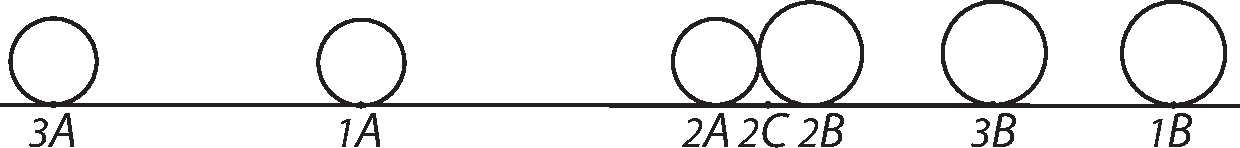
\includegraphics[width=0.67\textwidth]{%
gesamttex/edit_VIII,3/images/LH_37_05_144r-145v_d3_144r.pdf%
}} 
\vspace{0.5em}
\centerline{%
\lbrack\textit{Fig.~3}\rbrack%
}
% \newpage%
\vspace{1.5em}
%%%
\pstart
Nam ponamus \textit{A} esse minus et \textit{B} majus et concurrere in centro concursus%
\protect\index{Sachverzeichnis}{centrum concursus} \textit{{\scriptsize2}C}, aequali celeritate%
\protect\index{Sachverzeichnis}{celeritates aequales} ${\scriptstyle \textit{1}}A{\scriptstyle \textit{2}}A\, \sqcap\, {\scriptstyle \textit{1}}B{\scriptstyle \textit{2}}B$.  
%
Erit
%
\textit{{\scriptsize3}A{\scriptsize2}C}, ad \textit{{\scriptsize1}B{\scriptsize2}C} ut corpus \textit{B} ad corp.\ \textit{A} et \textit{{\scriptsize3}B{\scriptsize2}C} ad \textit{{\scriptsize1}A{\scriptsize2}C} ut corpus \textit{A} ad 
%
\edtext{corp.\ \textit{B}, hypothesi}{\lemma{corp.\ \textit{B}}\Bfootnote{\textit{(1)}~et quia in tali \textit{(2)}~, hypothesi~\textit{L}}}
%
ubi centrum concursus\protect\index{Sachverzeichnis}{centrum concursus} et %
punctum contactus\protect\index{Sachverzeichnis}{punctum contactus} idem. Imo omissa tali hypothesi, et 
%
\edtext{omiss\lbrack um\rbrack\ centr\lbrack um\rbrack}{%
\lemma{}%
\Bfootnote{%
omisso centro %
\textit{L ändert Hrsg.}%
}}
%
concursus%
\protect\index{Sachverzeichnis}{centrum concursus}\lbrack,\rbrack\ ex demonstratis\lbrack,\rbrack\ seu 
%
\textit{{\scriptsize3}A{\scriptsize2}A} ad \textit{{\scriptsize1}B{\scriptsize2}B}, ut corp.\ \textit{B} ad corp.\ \textit{A}, \textit{{\scriptsize3}B{\scriptsize2}B} ad \textit{{\scriptsize1}A{\scriptsize2}A} ut corp.\ \textit{A} ad corp.\ \textit{B}.  
%
Est autem ex hypothesi ${\scriptstyle \textit{1}}B{\scriptstyle \textit{2}}B \sqcap {\scriptstyle \textit{1}}A{\scriptstyle \textit{2}}A$. 
%
Ergo %
$\displaystyle\frac{i}{m} \sqcap \doublefrac{\displaystyle\frac{b}{a}f}{\displaystyle\frac{a}{b}e}$ %
 et $f\sqcap e$. Ergo $\displaystyle\frac{i}{m} \sqcap \displaystyle\frac{b^2}{a^2}$.
Ergo si duo %
corpora inaequalia\protect\index{Sachverzeichnis}{corpora inaequalia} aequali celeritate%
\protect\index{Sachverzeichnis}{celeritas aequalis} concurrant celeritates concursu quaesitae%
\protect\index{Sachverzeichnis}{celeritas concursu quaesita} sunt in ratione corporum reciproca duplicata%
\protect\index{Sachverzeichnis}{ratio reciproca duplicata}. Generaliter autem ex
%
$\displaystyle\frac{i}{m} \sqcap \doublefrac{\displaystyle\frac{b}{a}f}{\displaystyle\frac{a}{b}e}$, 
%
fiet 
%
$\displaystyle\frac{ei}{fm} \sqcap \displaystyle\frac{b^2}{a^2}$.
%
\edtext{Id est: Ratio}{\lemma{Id est:}\Bfootnote{\textit{(1)}~ante et \textit{(2)}~Ratio~\textit{L}}}
%
composita\protect\index{Sachverzeichnis}{ratio composita} celeritatum ante et post concursum\protect\index{Sachverzeichnis}{concursus} est eadem cum ratione corporum reciproca duplicata\protect\index{Sachverzeichnis}{ratio reciproca duplicata}.
\pend \pstart
%%%
Hinc illud praeclarum theorema%
\protect\index{Sachverzeichnis}{theorema praeclarum}: Si duo
%
\edtext{corpora quibuscunque}{\lemma{corpora}\Bfootnote{\textit{(1)}~quacun \textit{(2)}~quibuscunque~\textit{L}}}
%
celeritatibus concurrant, semper inveniemus eandem manere rationem compositam\protect\index{Sachverzeichnis}{ratio composita} ex ratione celeritatum\protect\index{Sachverzeichnis}{ratio celeritatum} ante concursum%
\protect\index{Sachverzeichnis}{ratio celeritatum ante concursum} cum ratione celeritatum post concursum%
\protect\index{Sachverzeichnis}{ratio celeritatum post concursum}. Hinc
%
\rule[0cm]{0mm}{16pt}%
$\displaystyle\frac{ei}{fm} \sqcap \displaystyle\frac{iv}{mw}$. 
%
Ergo
%
$\displaystyle\frac{e}{f} \sqcap \displaystyle\frac{v}{w}$.
%
\pend \pstart
%%%
Hinc novum 
\rule[0cm]{0mm}{10pt}%
theorema\protect\index{Sachverzeichnis}{theorema}: Si duo corpora bis concurrant, erunt celeritates ante primum concursum%
\protect\index{Sachverzeichnis}{concursus primus} proportionales celeritatibus post secundum%
\protect\index{Sachverzeichnis}{concursus secundus}. Videndum an non eaedem. Nam ac
%
$i \sqcap \displaystyle\frac{b}{a}f$\lbrack,\rbrack\ 
%
$m \sqcap \displaystyle\frac{a}{b}e$\lbrack,\rbrack\
%
$v \sqcap \displaystyle\frac{b}{a}m$,
%
et
%
$w \sqcap \ \displaystyle\frac{a}{b}i$.
%
\rule[0cm]{0mm}{16pt}%
Ergo $v \sqcap e$ et $w \sqcap f$. Ergo celeritates ante primum\protect\index{Sachverzeichnis}{concursus primus} et post 
\rule[0cm]{0mm}{10pt}%
secundum concursum\protect\index{Sachverzeichnis}{concursus secundus} eaedem.
\pend